% \documentclass[rnd]{mas_proposal}
\documentclass[thesis]{mas_proposal}

\usepackage[utf8]{inputenc}
\usepackage{amsmath}
\usepackage{amsfonts}
\usepackage{amssymb}
\usepackage{graphicx}

\title{Project Proposal Title}
\author{Lokesh Veeramacheneni}
\supervisors{Dr. Paul G Pl\"{o}ger\\ Dr. Matias Valdenegro Toro \\ Third Supervisor}
\date{Month 2021}

% \thirdpartylogo{path/to/your/image}

\begin{document}

\maketitle

\pagestyle{plain}

\section{Introduction}
% \begin{itemize}
%     \item An introduction to the general topic you are covering.
%     \item Why is it important?
% \end{itemize}
Many robotic [cite], autonomous driving [cite] systems deployed in real world, dynamic environments now use LiDAR as the primary sensor.
The 3D LiDAR data acquired offers a true-size replica of rich 3D geometry and can be represented as 3D point cloud format or using 2D grids. eg: range image representation [cite].
Semantic scene understanding is one of the key component of autonomous driving systems. 
Semantic segmentation is an important task in semantic scene understanding.
Semantic segmentation requires labelling of each datapoint (3D point in LiDAR/pixel in camera) with its corresponding class.

The existing models for 3D semantic segmentation are insanely complex and uncertain about their detections [cite]. 
This uncertainty in addition with input as out of distribution (OOD) object question the safety and performance of the models.
One such real world example is Tesla autopilot stops after misdetecting a billboard with "STOP" written on it as a traffic stop sign [cite]. 
Another such failure is the same autopilot detecting the moon as a yellow sign and slows the car [cite].
In all the above scenarios, the model is unable to detect the object as OOD and resulting in undesired outcomes.

A decade long studies has been performed on task of semantic segmentation, [cite 16] referrs to all the traditional approaches based on handcrafted features.
With the advent of deep learning, a richer feature representation led to mapping input to semantic labels as an end to end procedure.
The most popular 3D semantic segmentation datasets in the context of autonomous driving are Semantic KITTI [cite], nuScenes-lidarSeg [cite] and Sydney Urban [cite] collected by various sensors are publicly available.
3D semantic segmentation datasets are limited in size and diversity because labeling is intensive and requires special skill to handle.

There are diverse range of methods for the task of 3D semantic segmentation. 
They inlcude point based methods such as PointNet++ [cite], RandLA-Net [cite], and many more.
There also exists image based methods which employ various projection algorithms and popular methods in this segment include SqueeseSegV3 [cite], RangeNet++ [cite], and SalsaNext [cite].
Graph based and Voxel based methods are some of their own kind to solve the task of 3D semantic segmentation.
In the later sections, we will discuss about the problem statement, corresponding related work and project plan.


\subsection{Problem Statement}
% \begin{itemize}
%     \item What are you going to solve?
%     \item How are you evaluating?
% \end{itemize}


\section{Related Work}
\begin{itemize}
    \item What have other people done?
    \item Why is it not sufficient?
\end{itemize}

\subsection{Subsection 1}
\subsection{Subsection 2}



\section{Project Plan}
In this section, the project plan including work packages, tasks and timeline for each task is proposed.
\subsection{Work Packages}
The bare minimum will include the following packages:
\begin{enumerate}
    \item[WP1] Literature Search
    \begin{itemize}
        \item[-] Literature search on the existing 3D datasets on semantic segmentation for benchmarking.
        \item[-] Literature search on the existing  3D models for semantic segementation.
        \item[-] Literature search over the out of distribution methods.
        \item[-] Documentation.
    \end{itemize} 
    \item[WP2] Dataset OOD benchmark proposal
    \begin{itemize}
        \item[-] 3D semantic segmentation dataset collection for benchmarking.
        \item[-] Benchmark datasets for in-distribution and out-distribution.
        \item[-] Documentation.
    \end{itemize}
    \item[WP3] Experimentation
    \begin{itemize}
        \item[-] Implement an existing 3D semantic segmentation model as baseline model.
        \item[-] Implement the state of the art (SOTA) 3D semantic segmentation model
        \item[-] Extend the implemented 3D model (baseline and SOTA) to out of distribution detection problem.
        \item[-] Documentation. 
    \end{itemize}
    \item[WP4] Evaluation
    \begin{itemize}
        \item[-] Evaluate the baseline model and SOTA model on the proposed evaluation methods.
        \item[-] Compare both the model on OOD detection
        \item[-] Documentation
    \end{itemize} 
    \item[WP5] Project Report
    \begin{itemize}
        \item[-] Update and review existing report sections (literature, datasets, experimentation and evaluation)
        \item[-] Report completion and submission
    \end{itemize} 
\end{enumerate}
% Keep in mind that depending on your project, you will probably need to add work packages that are more suited to your projects.

\subsection{Milestones}
\begin{enumerate}
    \item[M1] Literature search
    \item[M2] Dataset benchmarking
    \item[M3] Models implementation
    \item[M4] Evaluation and comparison
    \item[M5] Report submission
\end{enumerate}

\subsection{Project Schedule}
% Include a gantt chart here. It doesn't have to be detailed, but it should include the milestones you mentioned above.
% Make sure to include the writing of your report throughout the whole project, not just at the end.
The detailed plan of tasks in duration of 6 months of thesis is given in figure [cite].

\begin{figure}[h!]
    \centering
    \caption{Illustration of project timeline}
    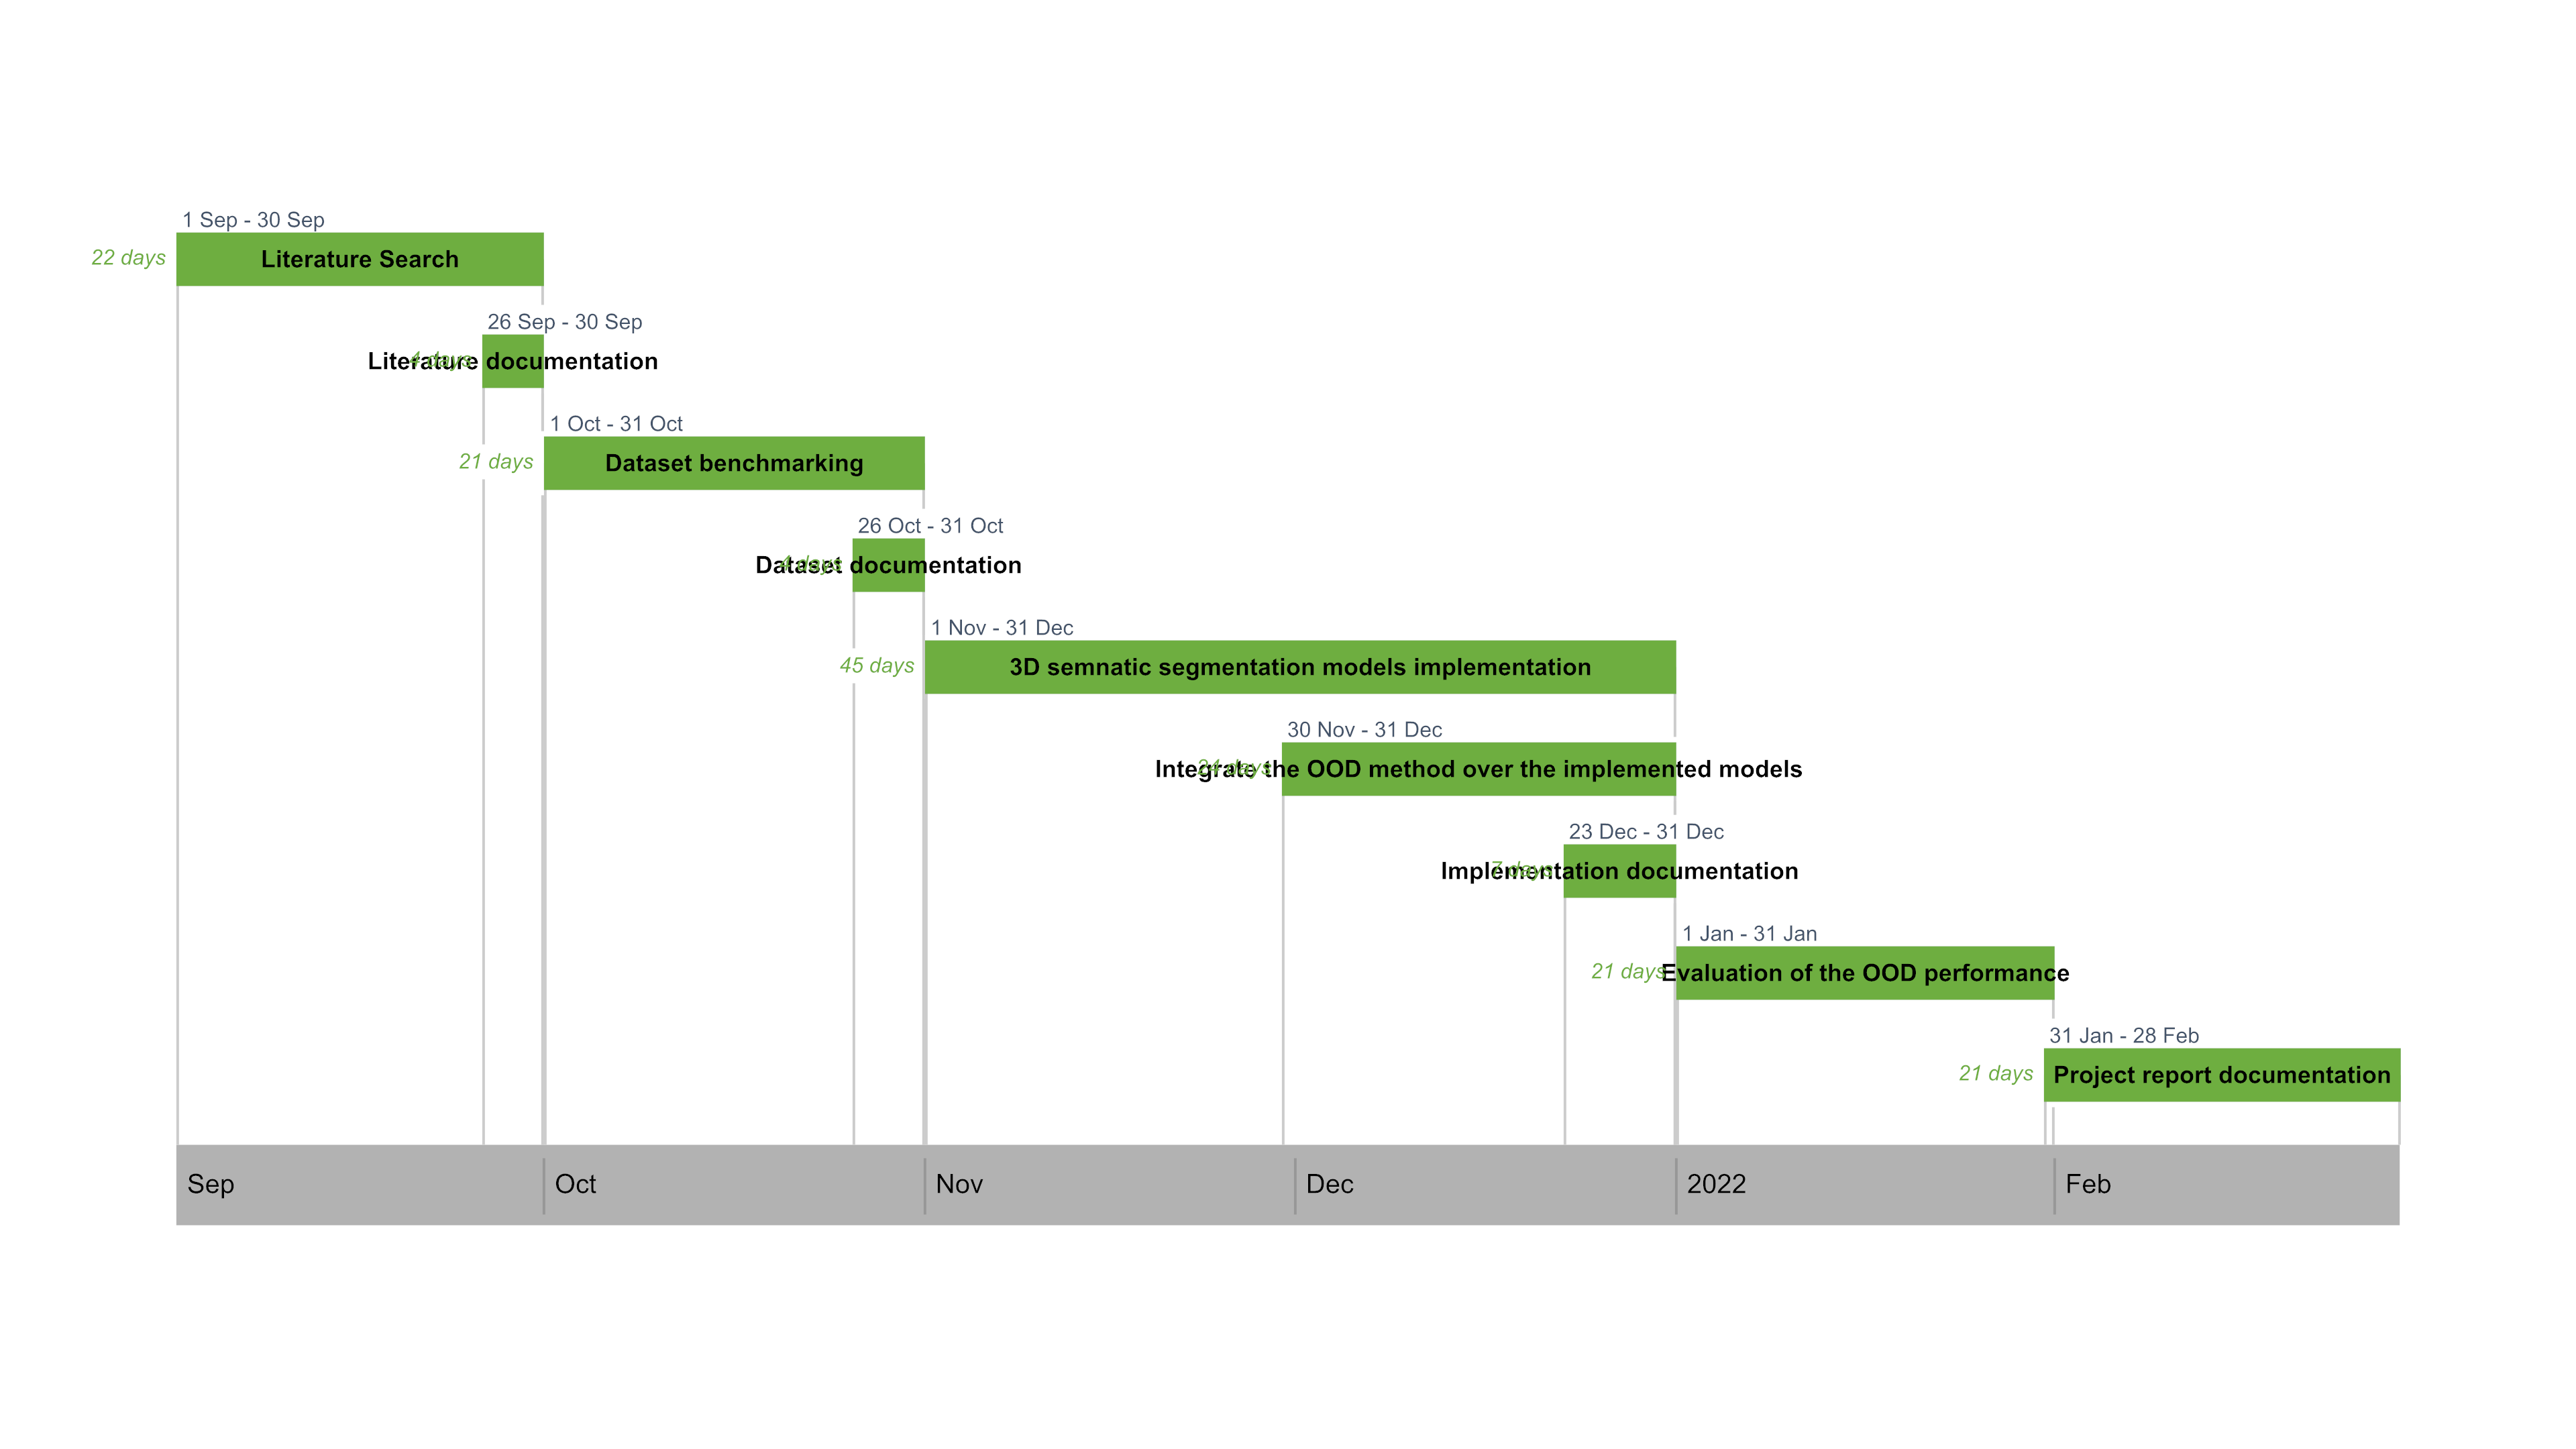
\includegraphics[scale=0.16]{images/rnd_deliverable_timeline}
    % 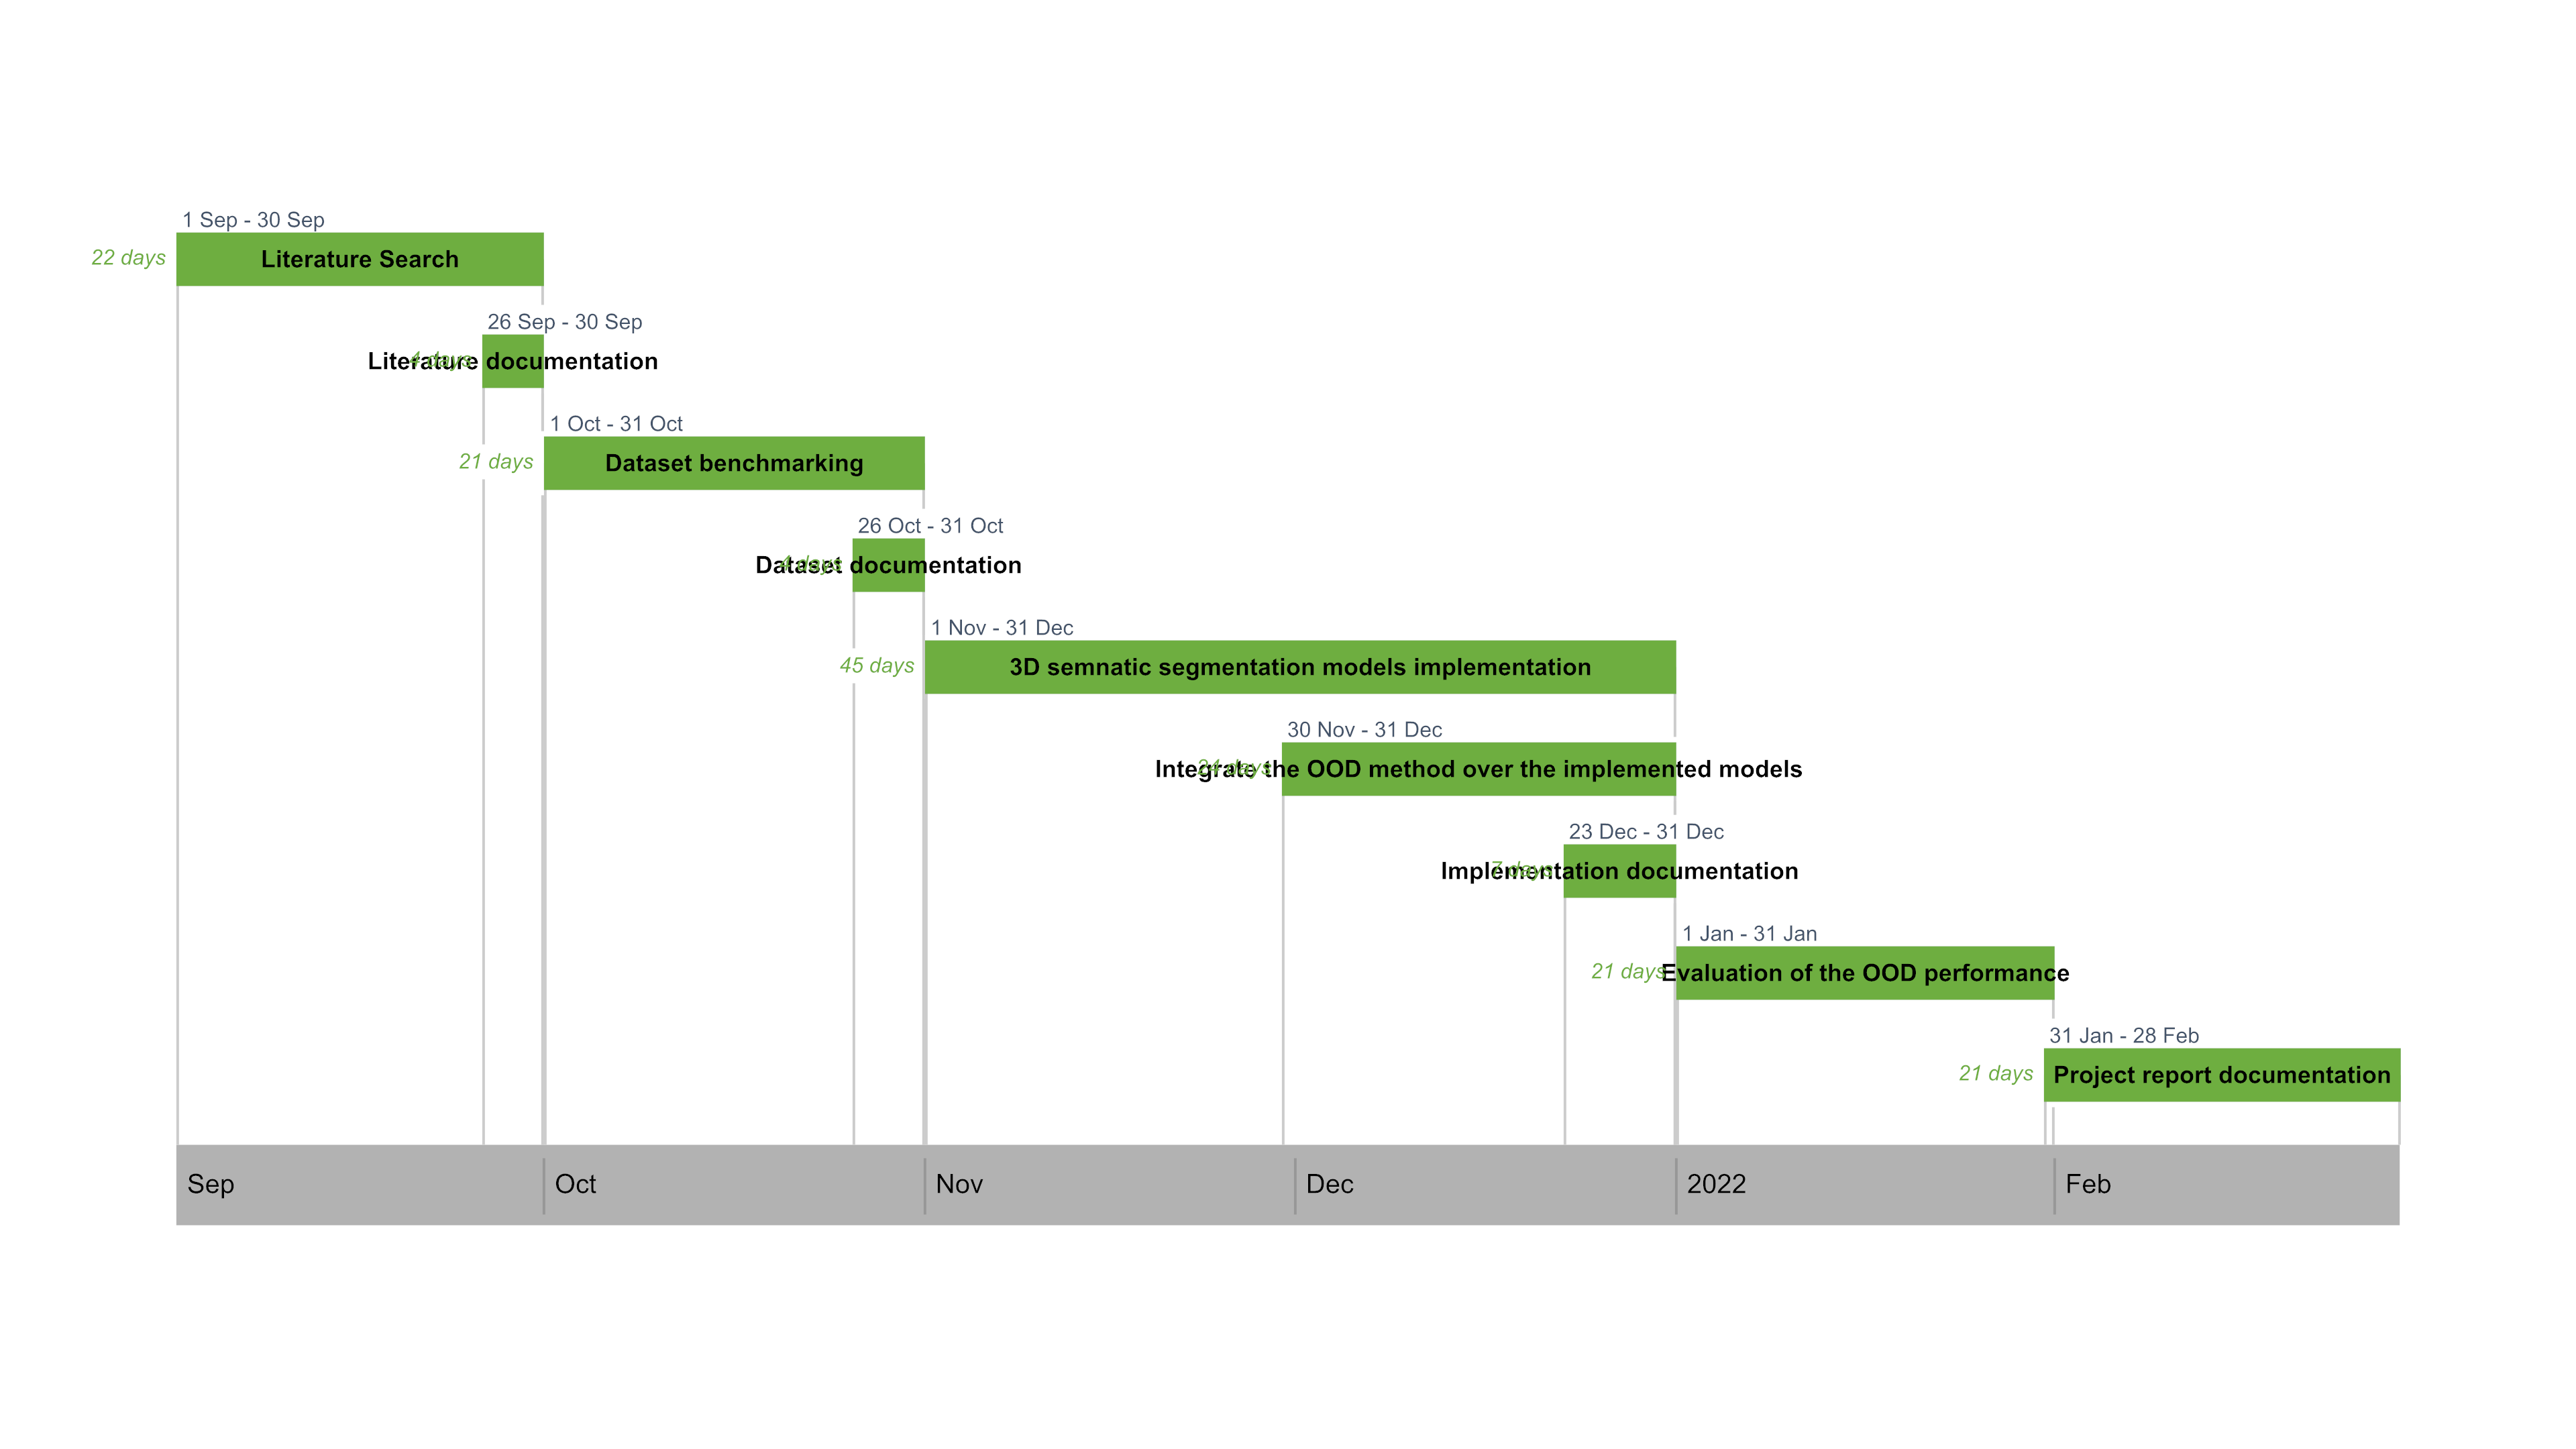
\includegraphics[width=\textwidth]{images/rnd_deliverable_timeline}
    \label{fig:schedl}
\end{figure}

\subsection{Deliverables}
\subsubsection*{Minimum Viable}

\begin{itemize}
    \item Systematic literature survey of methods over
        \subitem- Datasets in 3D LiDAR semantic segmentation
        \subitem- Existing out of distribution methods 
        \subitem- 3D models for semantic segmentation on LiDAR data
    \item Proposal of 3D benchmarking datasets for out of distribution detection
    \item Study of uncertainty estimation over 3D models for OOD detection
    \item Extension of OOD detection method to a baseline 3D model
\end{itemize}

\subsubsection*{Expected}
\begin{itemize}
    \item Systematic evaluation of the implemented baseline model over the benchmarked dataset
    \item Implementation of the state of the art model for OOD detection
    \item Evaluation and comparison of the implemented state of the art model to baseline algorithm
\end{itemize}

\subsubsection*{Desired}
\begin{itemize}
    \item Proposal of a refinement over the current OOD model for higher performance
\end{itemize}


\nocite{*}

\bibliographystyle{plainnat} % Use the plainnat bibliography style
\bibliography{bibliography.bib} % Use the bibliography.bib file as the source of references




\end{document}
